\documentclass{article}

% page stuff
\setlength{\topmargin}{-.3 in}
\setlength{\oddsidemargin}{0in}
\setlength{\evensidemargin}{0in}
\setlength{\textheight}{9.in}
\setlength{\textwidth}{6.5in}
\pagestyle{empty}

% delcare packages used
%\usepackage{bbold}
\usepackage{amsthm}
\usepackage{amsmath}
\usepackage{amsfonts}
\usepackage{amssymb}
\usepackage{algorithm2e}
\usepackage{graphicx}
\usepackage{float}
\usepackage{fancyvrb}
\usepackage{fancyhdr}
%\usepackage{wasysym}

% declare theorem environments
\newtheorem{thm}{Theorem}
\newtheorem*{claim}{Claim}
\newtheorem{mydef}{Definition}

\begin{document}

\title{Portfolio Playground  \\ CPSC 437 / 537 - Final Project}
\author{Chris Harshaw, Daniel Keller, Felipe Pires}
\date{\today}
\maketitle

\pagestyle{fancy}
\fancyhf{}
\rhead{CPCS 537 -- Final Report}
\lhead{Harshaw, Keller, Pires}
\rfoot{\thepage}



\section{Introduction}
Trading stock can be exciting and rewarding activity, both intellectually and monetarily. However, there is a significant barrier to entry as trading stocks requires a large investment. A solution to this problem is \emph{paper-trading}, simulated trading to practice buying and selling securities without actual money being involved. This allows novice investors to compare different buying and selling techniques without the risk of losing money. This practice is informative and worthwhile.

We present \textbf{\emph{Portfolio Playground}}, a paper-trading web application developed at Yale University. Portfolio Playground deals specifically with paper trading with stock portfolios. Not only does our application support portfolio creation and analysis, but also comparison between portfolios and even several state-of-the-art portfolio recommender algorithms. There are many other paper-trading apps on the market, each with different selling points. Apps such as ``Best Brokers: Stock Market Game'' and ``Wall Street Survivor'' involve game-ification aspects while ``TD Ameritrade'' offers users access to their world-class data and analytics. From our research, we believe that Portfolio Playground is the only paper-trading application to automatically recommend portfolios and freely release the source code.

In Section~\ref{sec:fun_walk}, we describe basic functionality and provide a simple walkthrough. We discuss our recommender algorithms in Section~\ref{sec:alg}, database design in Section~\ref{sec:db}, and front-end design in Section~\ref{sec:fe}. Finally, we discuss the main issues of our system in Section~\ref{sec:main_issues} and in Section~\ref{sec:division}, we discuss the division of labor.

\section{Functionality and Walkthrough} \label{sec:fun_walk}
The Portfolio Playground has three main functionalities:
\begin{enumerate}
	\item Portfolio creation and analysis
	\item Portfolio comparison
	\item Portfolio recommendation
\end{enumerate}
In the remainder of this section, we provide a walkthrough tutorial on how to explore the application's functionality. Before we continue, however, we provide a brief introduction to the portfolio metrics that are used in the application.

Suppose we have a portfolio $P$ consisting of stocks $P = \{s_1\dots s_N\}$, where $x_i$ is the number of shares of stock $s_i$, $D_i$ is the dividends for stock $s_i$, and $P^{t}_{i}$ is the price of a single share of stock $s_i$ at time $t$. Then we can define the \emph{total stock return} (TSR) from a stock creation time $t_0$ to a later time $t_f$ as 

$$TSR = \sum_{i=1}^N x_i \left( \frac{P^{t_f}_{i} - P^{t_0}_{i} + D_i}{P^{t_0}_{i}} \right) $$

Total stock return is a well-accepted metric used commonly in econometrics. Intuitively, the total stock return is a weighted percent increase function over the portfolio. A more colloquial term is the `diversity' of a portfolio. A portfolio is said to be diverse if the stocks contained therein are robust to changes in the other stocks. We rigorously define the \emph{diversity} of a portfolio as

$$Div = 1 - \frac{1}{Z} \sum_{i<j}^N x_i x_j Cor(P_i,P_j) \in \left[ 0,1 \right]$$

where $Z$ is a normalization term $Z = \sum_{i<j}^N x_i x_j$. Intuitively, the diversity of a portfolio is a weighted correlation score, where the weightings are derived from the number of shares owned in a particular stock. These two metrics are used frequently in our portfolio analysis and comparison. We now provide a brief walk-through tutorial of Portfolio Playground.


\section{Recommender Algorithms} \label{sec:alg}
Perhaps the most interesting and novel feature of Portfolio Playground is the portfolio recommendation algorithms. In this section, we describe these algorithms in detail. At the end of the section, we point out potential flaws in these algorithms and why they do not arise in our applications. Our recommendation algorithms make use of vector autoregressive models. We assume that our audience is familiar with these models (indeed, Ennan expressed that he was familiar with VAR models during our presentation). If this is not true, we encourage the interested reader to peruse Chapter 11 of "Time Series Analysis" by James D. Hamilton.

\subsection{Random}
The random portfolio recommendation algorithm recommends a random portfolio under given budget constraints. At each step of the algorithm, a random stock and number of shares are chosen subject to budget constraints until the budget has been met. A short description of the algorithm is given below.

\begin{enumerate}
	\item Initialize portfolio $P = \emptyset$
	\item Until budget constraints active,
		\begin{enumerate}
			\item $P \leftarrow P +$ random stock, random number of shares (under budget constraint)
		\end{enumerate}
\end{enumerate}

Note that the random algorithm generates a portfolio that can used as a ``control'' portfolio in experiments. In fact, these random portfolios can be used to test the ``Efficient Market Hypothesis''.

\subsection{Highest Return}
The highest return portfolio recommendation algorithm recommends a portfolio that maximizes expected total stock return (TSR) under budget constraints such as total budget and maximum investment per stock. First, a vector auto-regressive model (VAR) is fit to the data, using cross validation for parameter selection. Next, stocks are greedily added to the portfolio until the budget has been met. A short description of the algorithm is given below.

\begin{enumerate}
	\item Fit a Vector Autoregression Model to historical stock data
	\item Forecast the stock prices $d$ days away
	\item Initialize portfolio $P = \emptyset$. 
	\item Until budget constraints active,
		\begin{enumerate}
			\item $P \leftarrow P +$ stock that maximizes TSR
		\end{enumerate}
\end{enumerate}

\subsection{Diverse Option}
The diverse option recommendation algorithm recommends a portfolio that maximizes expected total stock return under \emph{diversity} and budget constraints. The diverse options is very similar to highest return except the stocks are chosen from those that are diverse with respect to the current portfolio. First, a VAR is fit to the data, using cross validation for parameter selection. At each step of the algorithm, we identify a set $A$ of stocks which are diverse with respect to the current portfolio and select the stock from $A$ which maximizes TSR. A short description of the algorithm is given below.

\begin{enumerate}
	\item Fit a Vector Autoregression Model to historical stock data
	\item Forecast the stock prices $d$ days away
	\item Initialize portfolio $P = \emptyset$. 
	\item Until budget constraints active,
		\begin{enumerate}
			\item $A = \{s \ | \ corr(s,x) < \sigma \ \forall \ x \in P\}$ (options diverse from $P$)
			\item $P \leftarrow P +$ stock from $A$ that maximizes TSR
		\end{enumerate}
\end{enumerate}

\subsection{Potential Flaws}
There are a few potential flaws in our recommendation algorithms, but they are mainly theoretical and not of any real practical concern here. Note that maximizing total stock return is exactly an instance of the knapsack problem. Indeed, we can only choose integral variables (i.e. we can't take 3/4 share of a stock) and our budget is limited by the current prices. Clearly, the optimizing total stock return is NP-Hard. 

We considered using clever integer programming methods for maximizing total stock return, but determined that a greedy algorithm worked reasonably well. Indeed, the greedy algorithm can perform arbitrarily poorly on general knapsack instances. However, this occurs when objects have wildly different values and costs. Fortunately, stocks do not have this worst-case property and so the greedy algorithm should perform relatively well at a much lower computational cost.

\section{Database Design} \label{sec:db}
In order to build Portfolio Playground and provide the data for the various recommendation algorithms it employs, we needed to determine which data we needed, find it, and then store it in a way that computations would not be repeated or take excessive amounts of time.  This section on database design will detail the choices we made with regard to which data we wanted, how we found it, and how we designed our database.

\subsection{Data Specification}
First and foremost, we must discuss the actual data we needed.  Looking at our use cases, you can see that we wanted to show value of stocks over time, total stock return of a portfolio over time, and diversity of a portfolio over time.  We also wanted a user to be able to create, track, and compare several different portfolios composed of different sets of stocks.  

In order to fulfill our first use cases, we needed to find the value of various stocks over long time periods.  In order to do this, we needed to get real data from the stock market.  While there are various websites that publish data for public use on different stocks, these websites have very strict terms of use statements that forbid web crawling or data scraping.  Due to this, we could not use rudimentary data scraping without paying hefty license fees.  However, we still needed a large amount of data to make our recommendation algorithms worthwhile.  How could we get around this problem?

\subsection{Data Collection}
Our answer was Tiingo API.  Tiingo is fintech startup that tries to provide Bloomberg quality data at a fraction of a price.  While they offer IEX, a much more comprehensive API that provides real time stock data, we didn’t need this information.  We only needed daily values, which was thankfully provided by a free to use API.  Using this API, we were able to get a stock’s daily low, high, close, open, and volume sold. The API also provided other daily information such as splits and dividends, and provided adjusted price values that would account for these edge cases. Using Tiingo, we could access all of the price data for each stock that we needed.

With the stock price data, we could then aggregate daily values and use them to compute values such as diversity and total stock return for portfolios.  These values were computed using libraries such as \texttt{numpy} and \texttt{statsmodels} to handle the large amounts of information we needed.  For example, daily portfolio diversity was computed by finding the covariance of stocks over a two month window.  Using a \texttt{numpy} array, it was relative easy to create one array and then shift the frame of reference as each day was computed instead of generating a new array for each computation.

\subsection{Database Architecture}
Now that we had our data, we needed a way to store it.  While it would be possible to query the API every time we needed information, this would have led us to building a very slow website.  Instead, we structured a database to store daily values for stocks and portfolios, allowing us to only fetch or compute values once.  See our ER diagram, shown below in Figure~\ref{fig:db_diagram}

\begin{figure}[H]
\begin{center}
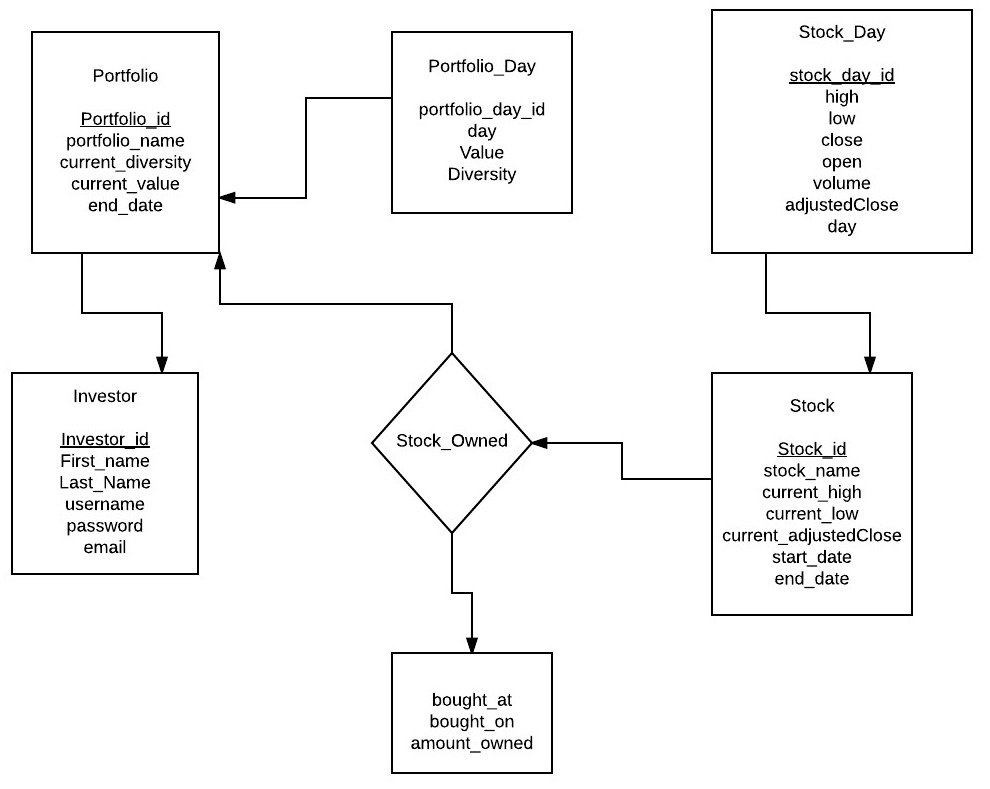
\includegraphics[width=0.7\textwidth]{db_diagram}
\caption{\label{fig:db_diagram} ER Diagram of Portfolio Playground Database}
\end{center}
\end{figure}

Both the \texttt{Portfolio} and \texttt{Stock} entities have one to many relationships with \texttt{Portfolio\_Day} and \texttt{Stock\_Day} objects. These \texttt{*\_Day} objects function as weak entity sets. While they do not have all the data required to establish what they are, their relationship with their parent entity solves that issue. The \texttt{Portfolio} and \texttt{Stock} entities both store current values in them (i.e. \texttt{Portfolio} stores most recent diversity, \texttt{Stock} stores most recent \texttt{adjustedClose}) as a way to cache values. Often, we needed to find the current price of a stock or the current diversity of a \texttt{Portfolio}, but querying for all the days and then finding the most recent one would be unnecessary computation. Therefore, as days are added, the \texttt{Portfolio} and \texttt{Stock} entities related to those days have their cached values updated.  \texttt{Portfolio} and \texttt{Stock} entities also store an \texttt{end\_date} value.  This value is used for determining when a \texttt{Stock} or \texttt{Portfolio} needs to fetch or compute new values and make new \texttt{*\_Day} objects.  

These \texttt{*\_Day} objects allowed us to query for specific days instead of sorting through massive arrays, decrease the size of the parent entity, and use the database to order our results instead of sorting them ourselves.  Therefore, establishing weak entity sets was a good way to increase the speed and utility of our website.

\texttt{Stock} and \texttt{Portfolios} also needed to be connected since we needed to store data on how many stocks were in each portfolio.  In order to do this, we established a many-to-many entity set between \texttt{Stocks} and \texttt{Portfolios} named \texttt{Stock\_Owned}.  This entity set included additional data such as amount purchased, the price at which stocks were purchased, and the day on which stocks were purchased.  This allowed us to store important information about Portfolios and which stocks they owned.

Finally, we wanted to allow users to create accounts and save their portfolios over extended periods of time.  To make this happen, we created an investor entity which linked to Django’s default user entity and stored crucial information for authentication and stored relationship information to portfolios.


\section{Front-End Design} \label{sec:fe}
Discuss design discussions in front-end design.

Describe which tools were used.

\section{Main Issues} \label{sec:main_issues}
Data fidelity was the main issue that we faced - both missing data and multiple inconsistent data points. For instance, sometimes the Tiingo API would be not have stock prices for certain days. There were also instances where Tiingo API returned several prices for a stock on a given day. This is likely a result of the aggregation of the sources that they pull from, such as Quotemedia and Quandl. The issues of missing and multiple data points pose a serious threat to the success of our recommendation algorithms.

To overcome these issues, we implemented data cleaning methods at several levels. First, when multiple stock prices were returned for a single day and stock, we removed all but the most recently pulled price. In this way, we cleaned our database as inconsistencies were found. Moreoften, it was the case that we were missing data. For instance, only a few stocks reported prices on Thanksgiving Day 2016. Our data cleaning method for dealing with missing data was handled on the front end and involved either (i) interpolating data (ii) throwing away entire days / stocks in computations. Essentially, if only few data points were missing, then the data was interpolated. On the other hand, if a sufficiently large amount of data was missing, then we completely removed a single day or a single stock in our computations. This front-end data cleaning method resulted in clean and well-founded computations.

Our system has several limitations. First, we only supported \emph{static} portfolios. That is, our current framework assumes that stocks are added into a portfolio and kept there indefinitely. We do not support the ability to buy and sell stocks within a portfolio. Fortunately, our framework can be generalized to support dynamic portfolios. without too much trouble. The second system limitation is the sacalability of our forecasting models. We currently use Vector Autoregression Models (VAR), whose parameters grow quadratically in the number of stocks used. For this reason, we only recommend portfolios from the most popular stocks. A more scalable algorithm would allow us to recommend portfolios from a larger range of stocks. A third limitation is the time it takes to pull stocks from the API. Pulling a few stocks is quite fast but the first instantiation of the database takes quite a long time.

\section{Division of Labor} \label{sec:division}
Chris Harshaw did the initial domain research to understand relevant models, metrics, and methods. Chris proposed the high level view of the app, developed and implemented the recommender algorithms, developed back-end interfaces, wrote data-cleaning methods, and helped to debug back-end issues.  Daniel Keller carried out the initial research to determine which API to use to gather stock prices. Daniel designed the database, wrote the database code, debugged back-end issues, and wrote initial front-end code. Felipe Pires implemented the finalized front-end user interface. Chris wrote the presentation, and Chris and Danny wrote the final report.

\end{document}
